  \iftoggle{portrait}{
    \begin{multicols}{2}
  Visual servoing is an approach for controlling the motion of a robotic system from visual measurements \cite{chaumette2006visual}. The trifocal tensor is well known in computer vision for tracing geometric information from three images of the same scene \cite{Hartley2004}.  The trifocal tensor geometric model is more robust than the two view geometry models as it involves the information given by a third view, and the set of correspondences obtained is more robust to outliers.
 {\centering 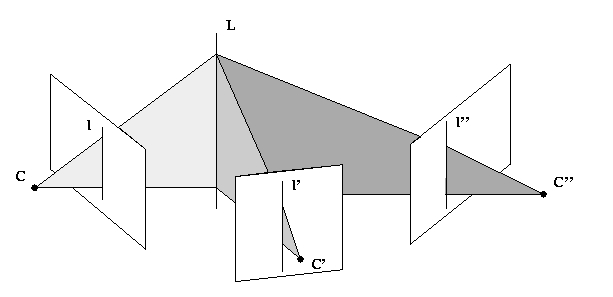
\includegraphics[width=.45\textwidth]{figures/threeviews.jpg}
 }\\
 Let the Camera positions be $C_{c^*},C_c,C_i$ for the desired, current, and initial camera positions respectively. And their projection matrices are $[I | 0]$, $[ ^{c}{\bf R}_{c^*} | ^{c}{\bf t}_{c^*} ]$, $[ ^{i}{\bf R}_{c^*} | ^{i}{\bf t}_{c^*} ]$. The Tensor relationfor calibrated cameras can then be expressed as follows:
$$
\mathcal{T}_{(jkl)} = \tensor[^{c}]{R}{_{c^{*}(kj)}} \ \tensor[^{i}]{t}{_{c^{*}(l)}} - \tensor[^{c}]{t}{_{c^{*}(k)}} \ \tensor[^{i}]{R}{_{c^{*}(lj)}}
$$
The trifocal tensor can be computed from feature correspondences across the three views \cite{Hartley2004}. Each triplet of corresponding image points gives 4 equations linearly independent. Therefore, a minimum set of 7 correspondences of points are needed for the trifocal tensor computation to uniquely determine the 27 entries of the tensor matrix.
  \end{multicols}
}{
Visual servoing is an approach for controlling the motion of a robotic system from visual measurements \cite{chaumette2006visual}. The trifocal tensor is well known in computer vision for tracing geometric information from three images of the same scene \cite{Hartley2004}.  The trifocal tensor geometric model is more robust than the two view geometry models as it involves the information given by a third view, and the set of correspondences obtained is more robust to outliers.
{\centering 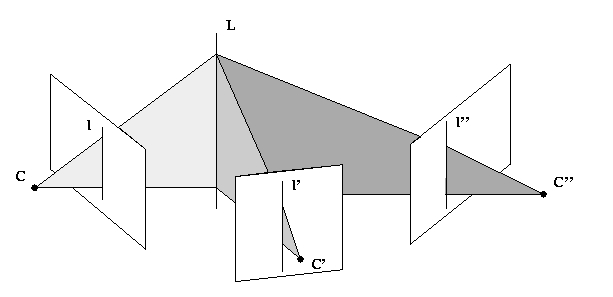
\includegraphics[width=.9\textwidth]{figures/threeviews.jpg}
}\\
Let the camera positions be $C_{c^*},C_c,C_i$ for the desired, current, and initial camera positions respectively, and their projection matrices be $[I | 0]$, $[ ^{c}{\bf R}_{c^*} | ^{c}{\bf t}_{c^*} ]$, $[ ^{i}{\bf R}_{c^*} | ^{i}{\bf t}_{c^*} ]$. The Tensor relation for calibrated cameras can then be expressed as follows:
$$
\mathcal{T}_{(jkl)} = \tensor[^{c}]{R}{_{c^{*}(kj)}} \ \tensor[^{i}]{t}{_{c^{*}(l)}} - \tensor[^{c}]{t}{_{c^{*}(k)}} \ \tensor[^{i}]{R}{_{c^{*}(lj)}}
$$
The trifocal tensor can be computed from feature correspondences across the three views up to a scale factor \cite{Hartley2004}. Each triplet of corresponding image points gives 4 equations linearly independent. Therefore, a minimum set of 7 correspondences of non-planar points are needed for the trifocal tensor computation to uniquely determine the 27 entries of the tensor matrix.
}
